\chapter{需求对话识别模型验证与分析}
本章目的在于对模型参数进行定量分析、通过把FRMiner与近年先进的需求识别基准方法和常见文本分类模型的效果对比验证孪生网络在复杂对话分类中的有效性以及FRMiner在跨项目实验中的表现,并分别介绍了以上实验的设置和实验结果说明和基本分析。

\section{验证实验设计}
这部分主要介绍我们设计的三个实验以及实验的基本设置。这三个实验都从三个开源项目数据集上使用了三折交叉验证\cite{DBLP:conf/ijcai/Kohavi95}。首先,我们随即将我们的数据集分成三部分,并使用其中两份作为训练集,剩下的一份作为测试集。我们重复这个过程三次,并且每次使用剩下的不同部分作为测试集。在三个实验中,均使用相同的分割数据集。另外,实验环境为Ubuntu操作系统,硬件配置为Intel core i7 CPU,16G RAM,NVIDIA 1060 GPU。
\subsection{FRMiner进行需求识别的有效性实验}
为了验证我们方法的有效性,我们针对从三个开源项目的聊天记录中进行特征请求对话识别实验进行了三折交叉验证。并且针对两个近年效果先进的在句子级别上分类为特征请求或者其他类别的分类器,我们与其比较了分类表现。由于原分类器的分类目标是句子,我们需要将其调整为对话级别的分类器,也即对话中包含为分类器预测为特征请求的句子时,我们认为该对话为特征请求对话。另外,我们和四个广泛使用的文本分类方法,进行对比,以验证FRMiner在有限标注数据上进行自动特征请求对话识别的有效性。

前面我们介绍了近年软件工程领域在特征请求识别方面的研究工作,其中章节2.1中的CNN-based Classifier(CNC)\cite{Huang2018Automating}和Feature Request Analyser(FRA) \cite{shi2017understanding}在特征请求分类上达到较好的效果。我们选用其作为特征请求分类方面的基线方法。CNC是目前从在线问题报告的评论中进行句子分类的最优模型,其使用基于卷积神经网络的方法把句子分为七个类别:信息提供、信息寻找、特征请求、问题提出、问题发现、方面验证和无意义的语句。我们使用其中特征请求的类别来预测,即将包含特征请求句子的对话分类为特征请求对话。FRA是一个从在线问题追踪系统中把句子进行特征请求分类的最优的基于规则的模型,其使用81个规则将句子分为六个类别,我们及那个包含类别\textit{Intent}的句子的对话分类为特征请求对话,同时,不包含\textit{Intent}句子的对话为非特征请求对话。对于CNC和FRA,我们使用了对应文献中中提供的代码和模型。

四个基于机器学习的方式我们选用如章节2.4.5中所述的朴素贝叶斯(NB)\cite{mccallum1998comparison}、随机森林(RF)\cite{liaw2002classification}、梯度提升决策树(GBDT)\cite{ke2017lightgbm} 和FastText(FT)\cite{joulin2016bag} 作为基线方法。NB为一个简单的使用词袋模型和贝叶斯规则的文本分类模型,它通过先验概率和学习训练数据得到的条件概率得到句子的后验概率,也即,给定一个句子,它可以推断出句子在所有类别下的概率。RF是一个使用多个树构建的集成机器学习模型,每个树都为最后的分类结果做贡献。在训练RF时,我们设置树的最大深度为2。GBDT是另一个集成学习方法,和RF的不同在于它的树是通过前面树的残差来决定的。当训练GBDT时,我们设置初始学习率为1.0,树的最大深度为1。FT是基于一个结构上类似于word2vec的浅层神经网络的文本分类方法,我们在实验中训练100轮,并设置初始学习率为1.0,输入n-gram的窗口大小为2。对于四个文本分类模型,我们使用官方提供的包 \footnote{https://scikit-learn.org/stable/} \footnote{https://fasttext.cc/},并且提取了词频-逆文档频率(TFIDF)\cite{joachims1996probabilistic} 作为对话特征向量来进行对话文本分类。接下来,我们使用网格搜索来微调四个文本分类模型的参数,使其达到最优效果。
另外,在以上的基线模型中,我们均使用了随机上采样\cite{ling1998data}来解决数据集的类别不均衡问题。

\subsection{孪生网络在FRMiner中的有效性实验}
为了检验引入孪生网络而带来的效果提升,我们构建了p-FRMiner,其是一个3.1中构建的以Single-Instance为输入的基本上下文敏感对话分类模型。然后,我们将p-{\tool}和使用Pair-Instance作为输入的{\tool}进行效果对比。之后,我们逐渐增加Pair-Instance训练集的大小来检验模型效果提升和数据集增强的关系。

需要注意的是,p-{\tool}和{\tool}是不同的分类模型,其中,p-{\tool}是对话上下文敏感模型,并接受单个对话作为输入,其模型结构图如图\ref{fig:model}所示。
\begin{figure}[htbp]
    \centering
    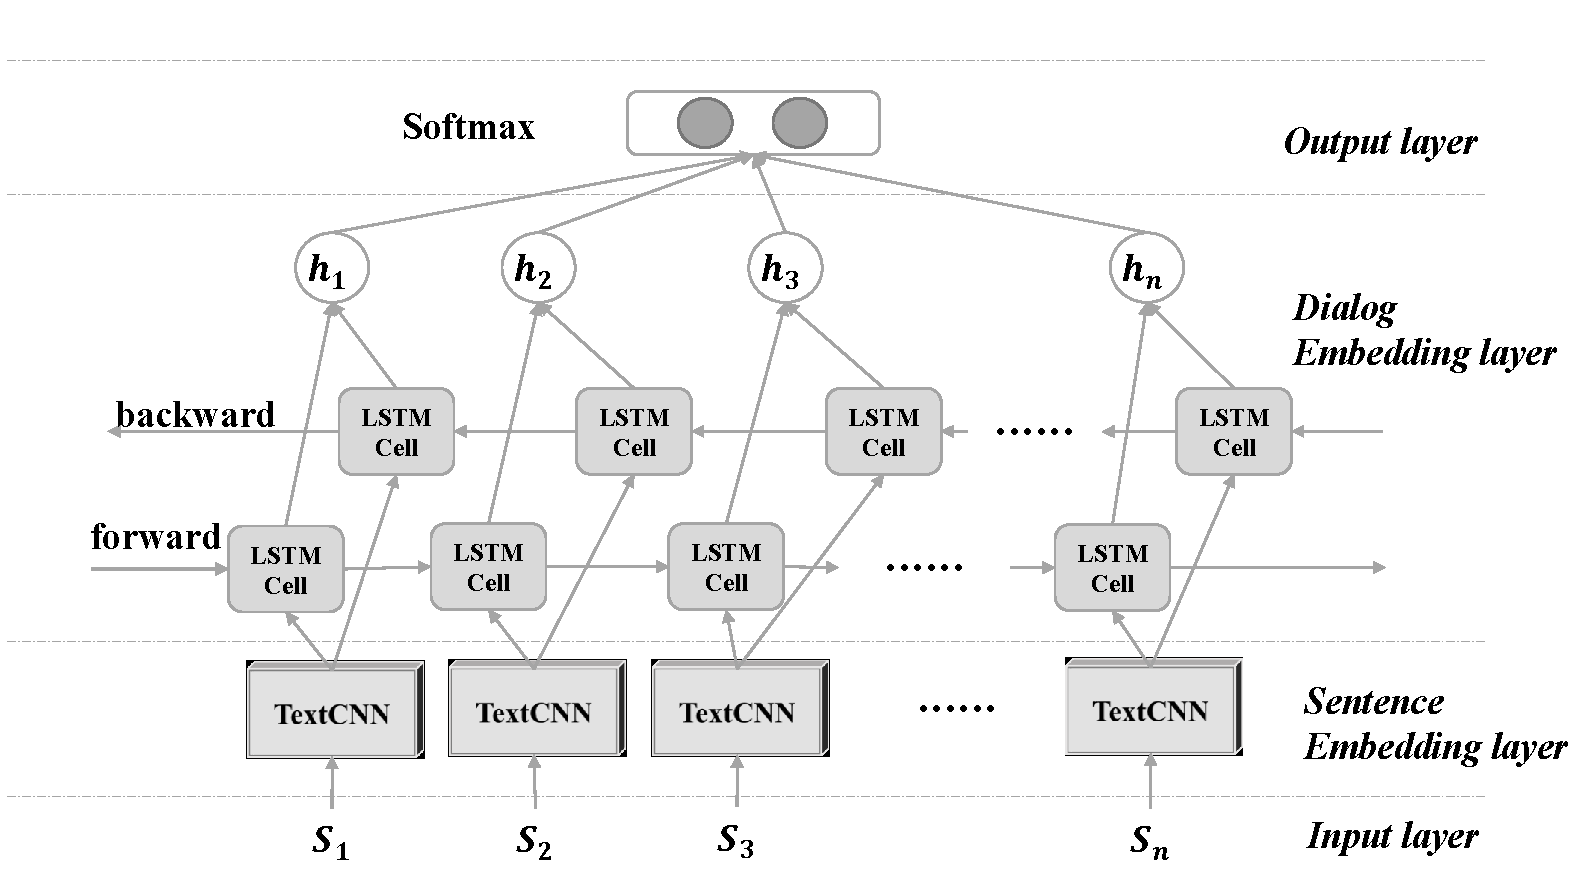
\includegraphics[width=\textwidth]{Img/model.pdf}
    \bicaption{p-{\tool}上下文敏感对话分类模型}{p-{\tool} Context-aware Dialog Classification Model}
    \label{fig:model}
\end{figure}
而{\tool}使用一对对话作为输入,其结构也可以通过修改p-{\tool}的结构得到。具体的,首先,移除p-{\tool}上层的分类层;拼接两个共享参数的相同的p-{\tool};最后,加上相似度度量层。

在实验部分,首先,我们使用相同大小的数据集来训练{\tool}和p-{\tool},并观察最后的效果增强。然后,我们把训练集分别增广到5倍、10倍、20倍和30倍来观察效果变化。因为{\tool}可以利用孪生网络天然的解决数据类别不均衡问题,然而,p-{\tool}不能,因此,我们通过随机上采样来均衡p-{\tool}的数据集。为了保证我们实验的准确性{\tool}和p-{\tool}使用相同的超参数进行训练,包括每层的维度,网络的深度以及学习率等。
\subsection{FRMiner的跨项目实验}
接下来,我们通过在三个开源项目数据集上验证了我们方法的泛化能力。我们迭代的使用其中两个项目作为训练集,剩下的一个项目作为测试集。为进行泛化能力对比,我们也在基线方法上进行跨项目实验。其中,实验中所用到的参数和实验5.1.2中保持一致。

\section{实验结果及分析}
\subsection{FRMiner进行需求识别的有效性实验结果及分析}
表格展示了每个项目三折交叉验证中不同方法达到的不同效果。
\begin{table}
\bicaption{每个项目在项目内通过不同方法取得的效果}{The performance achieved by different approaches for each project in intra-project validation}
    \label{tab:rq1}
    \centering
    \footnotesize% fontsize
    \setlength{\tabcolsep}{4pt}% column separation
    \renewcommand{\arraystretch}{1.2}%row space 
\begin{tabular}{|c|c|c|c|c|c|c|c|c|c|c|}
\hline
\multicolumn{2}{|c|}{\multirow{2}{*}{\diagbox{方法\qquad}{效果\qquad}}}   & \multicolumn{3}{c|}{AngularJS}                           & \multicolumn{3}{c|}{Bootstrap}                         & \multicolumn{3}{c|}{Chromium}                          \\ \cline{3-11} 
\multicolumn{2}{|c|}{}                           & Precision        & Recall           & F1               & Precision        & Recall           & F1               & Precision        & Recall           & F1               \\ \hline
\multirow{2}{*}{本文方法}        & FRMiner   & \textbf{90.28\%} & \textbf{89.73\%} & \textbf{90.00\%} & \textbf{86.28\%} & \textbf{88.78\%} & \textbf{87.52\%} & \textbf{89.00\%} & \textbf{87.00\%} & \textbf{88.00\%} \\ \cline{2-11} 
                                     & p-FRMiner & 31.71\%          & 54.17\%          & 40.00\%          & 50.00\%          & 47.80\%          & 48.98\%          & 14.00\%          & 44.00\%          & 20.00\%          \\ \hline
\multirow{2}{*}{已有研究方法}    & CNC       & 7.70\%           & 44.44\%          & 13.13\%          & 16.38\%          & 34.21\%          & 22.13\%          & 9.56\%           & 67.00\%          & 16.73\%          \\ \cline{2-11} 
                                     & FRA       & 13.67\%          & 80.33\%          & 23.35\%          & 23.00\%          & 48.67\%          & 31.00\%          & 12.00\%          & {81.00\%} & 20.00\%          \\ \hline
\multirow{4}{*}{文本分类方法} & NB        & 20.00\%          & 27.67\%          & 22.33\%          & 25.67\%          & {62.00\%} & 36.00\%          & 14.33\%          & 44.33\%          & 21.00\%          \\ \cline{2-11} 
                                     & GBDT      & 36.00\%          & 22.33\%          & 27.33\%          & 41.67\%          & 35.67\%          & 38.33\%          & 9.33\%           & 7.33\%           & 8.00\%           \\ \cline{2-11} 
                                     & RF        & 52.67\%          & 11.00\%          & 16.33\%          & 57.00\%          & 29.00\%          & 38.33\%          & 0.00\%           & 0.00\%           & NA               \\ \cline{2-11} 
                                     & FT        & 23.33\%          & 5.33\%           & 8.67\%           & 57.67\%          & 29.00\%          & 38.33\%          & 38.00\%          & 9.10\%           & 15.00\%          \\ \hline
\end{tabular}
\end{table}

其中,对于Precision、Recall、F1值最优的效果使用黑体标出。我们可以看到{\tool}在三个项目中均取得了最好的效果,平均精确度、召回率、F1值分别是88.52\%, 88.50\%, and 88.51\%。另外,p-{\tool}比所有的基线方法效果要好。表明了通过BiLSTM记忆上下文信息可以帮助从聊天记录中的文本分类任务。

对于两个句子级别的分类方法,CNN仅能取得17.33\%的平均F1值,主要是因为CNC是在问题评论语料库上训练得到的,而不是特征请求对话。然而,其依然能取得48.55\%的平均召回率,这表明在这两个领域里面应该存在着共有的分类模式。同时,基于规则的分类器FRA可以在六个基线方法中取得最高的平均召回率,其为70.00\%,并且在AngularJS和Chromium两个项目上分别可以取得80.33\%和81.00\%的召回率。虽然其精确度较低,但是FRA的预测结果包含大量真实的特征请求对话,这意味着对话信息中的特征请求句子也服从FRA的规则。另一方面,由于FRA使用基于规则的分类方法,而不是有监督的机器学习方法,FRA在挖掘大规模的聊天信息方面更加高效,并且,基于FRA较高的召回率这一优势,我们可以通过其解决标注数据初期的粗粒度召回问题。

对于四个文本分类方法,NB在其中取得了最好的效果。虽然RF取得了在四个方法里面取得最高的F1值-27.33\%,但其在Chromium项目上存在着欠拟合问题,即不能很好的建模训练数据,其原因主要在于Chromium项目数据集不充分,不能得到很好的训练并学习到相关模式。以下是本文提出的{\tool}在效果上大大超过四个传统文本分类模型的原因:
\begin{enumerate}
    \item 和传统的文本分类模型相比,神经网络模型具有更大的信息容量,尤其在建模复杂的对话模型上能取得较好的效果。
    \item 直觉上,模型分类两个对话的类别是否相似要比将每个对话分类为其类别更加容易进行学习。
    \item 由于数据集规模较小,文本分类模型存在在欠拟合问题,而由于{\tool}是一个pair-wise方法,可以将原数据集增广为较大规模,可以保证模型在充足的数据集上进行训练。
\end{enumerate}

总的来说,{\tool}效果上明显超过两个句子级别的特征请求分类方法和四个传统文本分类方法。由于CNC和FRA两个句子级别基线方法可以直接应用于聊天记录数据并且达到较高的召回率,他们在数据标注方面可以起到粗粒度召回的作用。

\subsection{孪生网络在FRMiner中的有效性实验及分析}

图\ref{fig:p-FR}展示了分别在相同数量的Single-Instance和Pair-Instance数据集上训练的p-{\tool}和{\tool}的效果。其中蓝色的条形图代表p-{\tool}的效果,其是在两折数据上训练的结果,训练数据量如图例所示。橙色的条形图代表使用孪生网络的{\tool}的效果,图例所示为Pair-Instance的数量。我们可以看到但训练样本量相同时,{\tool}比p-{\tool}取得了明显的较高的分类效果。{\tool}对于精确度、召回率、F1值分别平均提高了46.79\%,31.13\%,42.90\%。

\begin{figure}[htb]
\centering
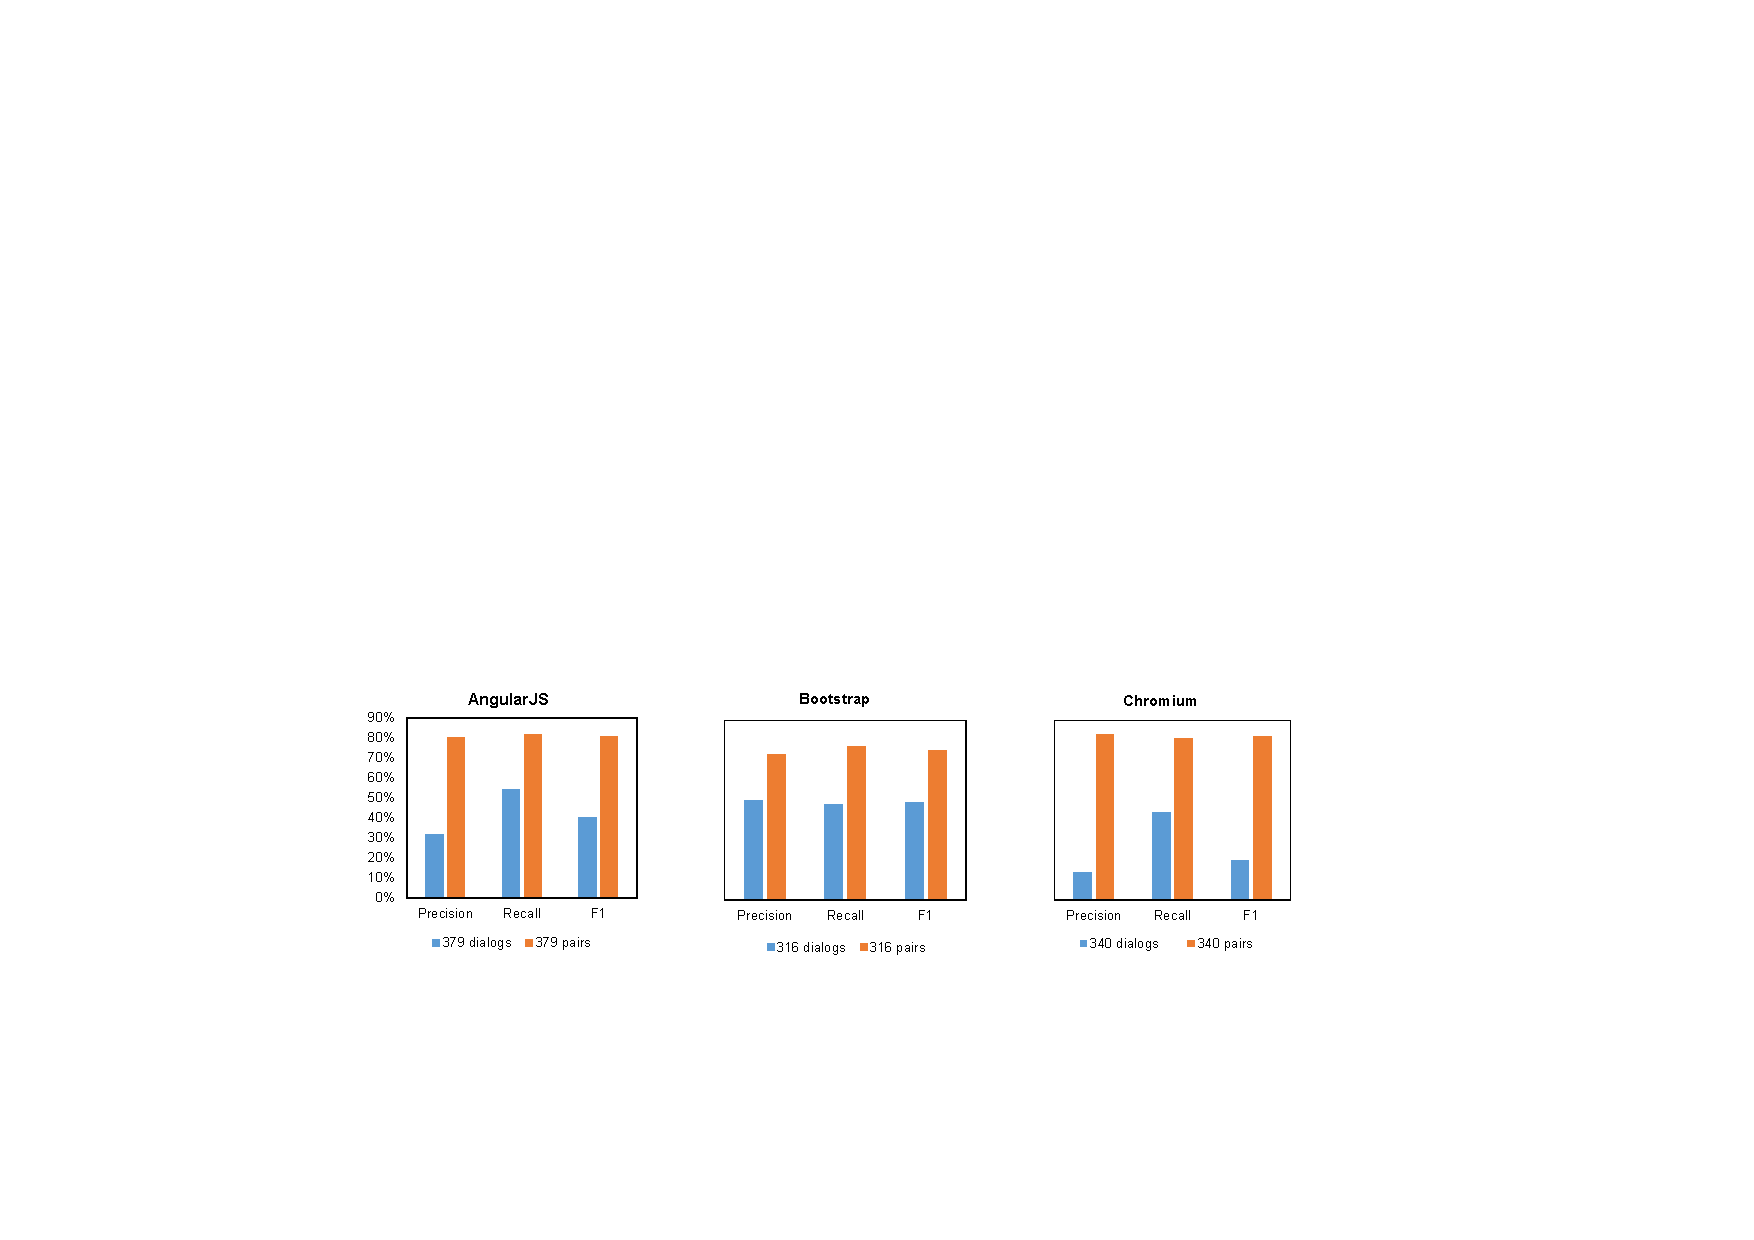
\includegraphics[width=\textwidth]{Img/p-FRvsFR.pdf}
\bicaption{p-FRMiner和FRMiner在相同大小训练集上的表现}{The comparison performances of p-FRMiner and FRMiner with the same volume of original training data}
\label{fig:p-FR}
\end{figure} 

图\ref{fig:FR-size}展示了Pair-Instance训练数据量的增广程度、分类效果的提升和在训练阶段花费的时间成本之间的关系。

\begin{figure}[htb]
\centering
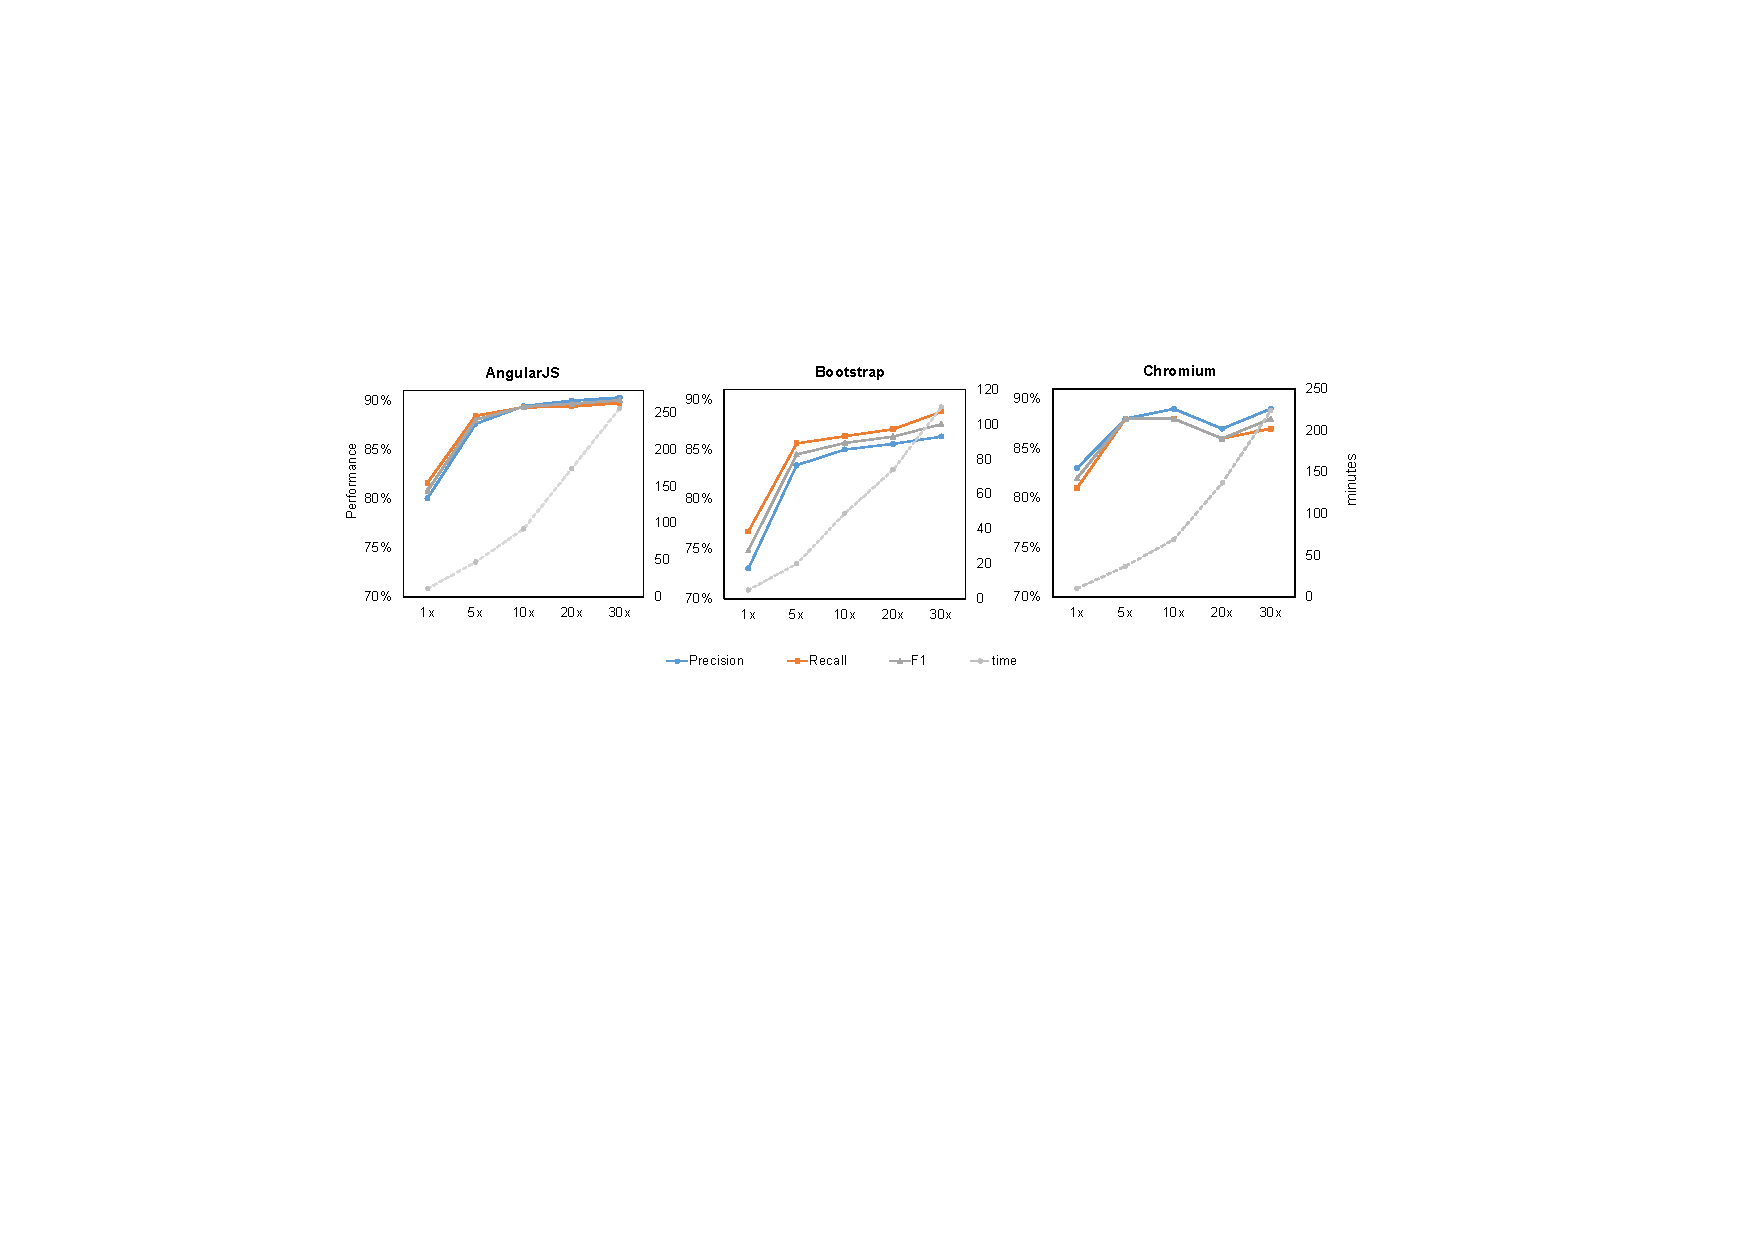
\includegraphics[width=\textwidth]{Img/FRMiner_size.pdf}
\bicaption{FRMiner在不同大小Pair数据集上的表现}{The performances of FRMiner when generating different numbers of pairs}
\label{fig:FR-size}
\end{figure} 

初始训练集数据量(1X数据量)如图\ref{fig:p-FR}所示,分别为379,316和340。我们可以看到通过扩大Pair-Instance训练集大小可以提高模型效果。当Pair-Instance训练集大小从1倍增广到30倍后,精确度、召回率、F1值分别平均提高了9.82\%,8.72\%和9\%。我们观察到模型效果在训练集扩大到5倍时提高最快,而从5倍增广到30倍时,三个项目上的效果提升较小。 当增广到20倍时,在Chromium项目上的效果甚至有较小的下降。而训练阶段所花费的时间基本呈现线性增加的特点。因此,我们认为将训练集增广到5倍是在训练效率和模型效果之间的一个较好的均衡的值。

总结来说,{\tool}比p-{\tool}可以更好地解决对话分类问题,在模型精确度、召回率、F1值上平均提升较大。实验结果表明了在训练数据较少的情况下,分辨两个对话是否同属于特征请求对话要比对单个对话分类为其类别更加简单。我们在实验中使用了5倍数据增广,因为更大的数据增强增加了模型训练时间成本,同时并不能带来更好的模型效果,而5倍数据增广较好的平衡了模型效果和训练时间成本。

\subsection{FRMiner的跨项目实验及分析}

表格\ref{tab:rq3}展示了在跨项目实验中每个项目作为测试集的表现。


\begin{table}[!htbp]
\bicaption{每个项目在跨项目实验中使用不同方法达到的效果}{The performance achieved by different approaches for each project in cross-project validation}
\label{tab:rq3}
    \centering
    \footnotesize% fontsize
    \setlength{\tabcolsep}{4pt}% column separation
    \renewcommand{\arraystretch}{1.2}%row space 
\begin{tabular}{|c|c|c|c|c|c|c|c|c|c|c|}
\hline
\multicolumn{2}{|c|}{}                                             & \multicolumn{3}{c|}{AngularJS}                                                                     & \multicolumn{3}{c|}{Bootstrap}                                                                   & \multicolumn{3}{c|}{Chromium}                                                                    \\ \cline{3-11} 
\multicolumn{2}{|c|}{\multirow{-2}{*}{\diagbox{方法\qquad}{效果\qquad}}}                    & Precision                      & Recall                         & F1                             & Precision                      & Recall                         & F1                             & Precision                      & Recall                         & F1                             \\ \hline
                                      & FRMiner                    & \textbf{85.23\%}               & \textbf{86.56\%}               & \textbf{85.89\%}               & \textbf{86.84\%}               & \textbf{85.89\%}               & \textbf{86.37\%}               & \textbf{85.87\%}               & \textbf{86.81\%}               & \textbf{86.34\%}               \\ \cline{2-11} 
\multirow{-2}{*}{本文方法}        & p-FRMiner                  & 31.03\%                        & 50.00\%                        & 38.30\%                        & 27.56\%                        & 69.08\%                        & 39.40\%                        & 16.00\%                        & 50.00\%                        & 24.24\%                        \\ \hline
                                      & {CNC} & {7.70\%}  & {44.44\%} & {13.13\%} & {16.38\%} & {34.21\%} & {22.13\%} & {9.56\%}  & {67.00\%} & {16.73\%} \\ \cline{2-11} 
\multirow{-2}{*}{已有研究方法}    & {FRA} & {13.67\%} & {80.33\%} & {23.35\%} & {23.00\%} & {48.67\%} & {31.00\%} & {12.00\%} & {81.00\%} & {20.00\%} \\ \hline
                                      & NB                         & 16.00\%                        & 75.00\%                        & 26.00\%                        & 27.00\%                        & 36.00\%                        & 31.00\%                        & 7.00\%                         & 26.00\%                        & 12.00\%                        \\ \cline{2-11} 
                                      & GBDT                       & 18.00\%                        & 14.00\%                        & 16.00\%                        & 30.00\%                        & 11.00\%                        & 16.00\%                        & 20.00\%                        & 19.00\%                        & 19.00\%                        \\ \cline{2-11} 
                                      & RF                         & 28.00\%                        & 14.00\%                        & 19.00\%                        & 37.00\%                        & 9.00\%                         & 15.00\%                        & 12.00\%                        & 26.00\%                        & 16.00\%                        \\ \cline{2-11} 
\multirow{-4}{*}{文本分类方法} & FT                         & 32.00\%                        & 19.00\%                        & 24.00\%                        & 43.00\%                        & 13.00\%                        & 20.00\%                        & 19.00\%                        & 11.00\%                        & 14.00\%                        \\ \hline
\end{tabular}
\end{table}

其中,最优的精确度、召回率、F1值使用黑体表示。需要注意的是,因为CNC和FRA是基于各自数据集训练的模型或者提取的规则,其不适用于跨项目实验,因此CNC和FRA的效果和5.1.1中项目内三折交叉实验的结果相同,为了对比和分析,我们将表格\ref{tab:rq1}中的数据复制到表格\ref{tab:rq3}中。我们可以看到{\tool}在跨项目实验中表现较好。平均F1值仅相比5.1.1中项目内实验降低2.27\%。其主要原因在于不同项目中表达特征请求的对话存在着共有的模式,并且可以在项目间进行共享。实验结果表明{\tool}可以学习到特征请求相关的范式,并且可以泛化到其他项目中,这表明开发者在不同的社区和项目中使用相似的模式表达特征请求。对于p-{\tool},其平均F1值相比项目内实验降低了10.51\%。

对于四个文本分类基线方法,NB取得了最高的F1值-23\%,并且相比项目内实验仅降低了3.44\%。我们注意到大多文本分类方法的模型效果在Angular和Chromium两个项目上比项目内实验要高,其主要是由于以下原因:
\begin{enumerate}
    \item 交叉项目实验中的训练数据集包含两个项目的数据集,而项目内实验仅包含一个项目的2/3大小的数据集。交叉项目实验可以在更充分的训练数据上进行训练。
    \item 由于交叉项目实验包含两个项目的数据集,更广泛领域的数据集可以通过引入不同领域的偏置信息帮助分类器增加泛化能力。
\end{enumerate}

因此,{\tool}在未训练数据集上依然能取得较好的效果,这表明{\tool}在不同项目见具有较好的泛化能力。同时,NB是在所有文本分类方法中从聊天记录中挖掘特征请求对话最好的方法。

\section{本章小结}

本章主要介绍针对我们提出的{\tool}设计了三个实验,包括{\tool}进行需求识别的有效性实验、孪生网络在{\tool}中的有效性实验以及{\tool}的跨项目实验的实验设置和参数配置。然后我们针对实验结果进行分析,试验结果表明我们的方法相较于两个句子级别的特征请求识别方法和四个文本分类方法有较大的性能提升,其中CNC和FRA召回率较高,在四个文本分类方法中NB的效果最好。另外由于开发者在不同项目之间通常使用相似的模式表达特征请求,因此对于捕获语法、语义能力较强的{\tool},其在跨项目中表现较好。